\documentclass[11pt]{article}
\usepackage[utf8]{inputenc}
\usepackage[T1]{fontenc}
\usepackage{lmodern}
\usepackage{enumitem}
\usepackage{amsmath,amssymb}
\usepackage{geometry}
\usepackage{graphicx}
\usepackage{xcolor}
\usepackage{listings}
\usepackage{hyperref}
\usepackage{tikz-cd}
\lstdefinelanguage{Rocq}{
  morekeywords={Fixpoint,match,with,end,fun,let,in,Theorem,
    Lemma,Proof,Qed,Definition,forall,exists},
  sensitive=true,
  morecomment=[s]{(*}{*)},
  morestring=[b]"
}
\geometry{margin=1in}
\setlist[itemize]{leftmargin=*}
\lstset{numbers=left,basicstyle=\small\ttfamily, columns=fullflexible,keepspaces=true, frame=single, breaklines=true, backgroundcolor=\color{gray!7}}

\title{Improving the Tactics \texttt{ring} and \texttt{field}\\
 }
\author{Thomas Portet}

\begin{document}
\maketitle

\begin{abstract}
This document describes an extension of Rocq's \cite{rocq-prover} reflexive algebraic tactics. The
main goal is to make \texttt{ring} and \texttt{field} usable on expressions that
contain functions outside the ring or field fragment. The approach rewrites the
arguments of such functions, computes polynomial greatest common divisors with
an OCaml oracle, and exposes the result to Rocq through ELPI foreign calls.
\end{abstract}
\section{Motivation}

We would like to formalize undergraduate mathematics in a style that remains close to ordinary pen-and-paper reasoning, while retaining the formal guarantees of a proof assistant. We therefore choose to work in a simple ambient theory, with a small collection of familiar mathematical objects and operations, and to allow users to express mathematical arguments through high-level declarative steps rather than low-level proof-assistant transformations.
\newline \newline
This setting motivates the question of how algebraic automation should behave when an algebraic expression occurs inside a function that is not itself part of the algebraic theory handled by the tactic. For example, a student should ideally be able to write

\[
\log(\pi^2+\pi\times\pi)=\log(2\pi^2)
\]
without having to explicitly expose the intermediate algebraic rewriting
\[
\pi^2+\pi\times\pi=2\pi^2.
\]
The proof assistant should be able to recognize and justify this transformation automatically.\newline
The difficulty is that the outer function $\ln$ is not a ring operation. Consequently, the algebraic tactic cannot treat the whole expression as a ring expression.

The existing \texttt{ring\_simplify} tactic addresses this issue for ring expressions by recursively simplifying algebraic expressions inside function applications.
% TODO: Here, the analogous example with log(\frac{2 \pi}{4}) = log (\frac(3 \pi}{6}) devrait être donné, en expliquant que field_simplify does not help as much as ring_simplify does in the other case
However, the analogous approach does not directly extend to field expressions. This raises the question of how to obtain a suitable representation of field expressions when they occur inside functions that the field normalizer does not handle.
\section{Reflexive Algebraic Normalization}
The starting point is the way Rocq's reflexive algebraic tactics normally solve
equalities. Rather than applying a sequence of rewriting lemmas, the tactic
reifies the input expression into an internal representation of the relevant
algebraic structure, computes its normal form, and uses this computation to
construct a proof. This approach is exemplified by the reflective ring tactic of Grégoire and Mahboubi \cite{gregoire2005proving}.


\subsection{Ring normalization}

The \texttt{ring} tactic works with integer constants, addition, multiplication, subtraction, and variables. Expressions outside this language are treated as fresh variables during reification. Thus, for an expression such as

$$
  \pi^2+\pi\mathbin{\times}\pi,
$$

the constant $\pi$ can be represented by a fresh variable $X$. The tactic then normalizes the resulting polynomial expression. When the normalized expression is reconstructed as a Rocq term, the fresh variable $X$ is replaced by the original expression $\pi$.

More generally, the process can be described in three steps:
\begin{enumerate}
\item reify the input expression, replacing supported operations by constructors in an internal polynomial representation and treating unsupported expressions as fresh variables;
\item normalize the resulting polynomial by collecting coefficients and combining like monomials;
\item conclude when the normalized expressions are syntactically equal.
\end{enumerate}


Although the arguments of the two logarithms are polynomial expressions, the complete terms

$$
  \log(\pi^2+\pi\mathbin{\times}\pi)
  \qquad\text{and}\qquad
  \log(2\pi^2)
$$

are themselves outside the polynomial language. At the level at which \texttt{ring} sees them, they therefore become distinct atoms. The tactic cannot discover that these atoms are equal by simplifying their arguments.

\subsection{Deep ring simplification}

The natural way to address this limitation is to apply ring simplification recursively inside function applications. Instead of treating an entire unrecognized function application as an indivisible atom, we first simplify the expressions occurring in its arguments and then reconsider the enclosing expression.

For example,

$$
  \cos(x+\cos(x+x))
  =
  \cos(\cos(2x)+(1-(1-x))).
$$

The relevant subexpressions include

$$
  x+\cos(x+x),\qquad
  x+x,\qquad
  \cos(2x)+(1-(1-x)),
  \qquad\text{and}\qquad
  2x.
$$

The inner expression $x+x$ can first be normalized to $2x$. The enclosing expression can then be reified again, with $\cos(2x)$ as an atom, allowing

$$
  \cos(2x)+(1-(1-x))
$$

to be normalized to

$$
  x+\cos(2x).
$$

The original equality consequently reduces to

$$
  \cos(x+\cos(2x))
  =
  \cos(x+\cos(2x)).
$$

This gives a natural recursive strategy for expressions containing unrecognized
functions: simplify their arguments, rebuild the function applications from
the simplified arguments, and continue at enclosing levels.

The same idea applies to the motivating logarithm example. The argument

$$
  \pi^2+\pi\mathbin{\times}\pi
$$

can be normalized to $2\pi^2$ before the surrounding $\ln$ application is considered. The two sides then contain the same function application, so the outer equality can be closed.

This approach works naturally for \texttt{ring} because polynomial normalization provides a canonical representation of the algebraic expression. For \texttt{field}, however, the situation is more subtle.

\subsection{Ring simplification versus field simplification}

The recursive strategy described above is implemented by \texttt{ring\_simplify}, which simplifies algebraic expressions inside function applications. An analogous approach using \texttt{field\_simplify} does not suffice for field expressions, as explained in the following section.

\section{The limits of {\tt field\_simplify}}
Consider
\[
  \frac{\pi}{\pi^2+\pi^2}=\frac{1}{2\pi}.
\]
\texttt{field} can prove this if it proves $\pi^2+\pi^2\ne0$ and
$\pi\ne0$.
In practice, \texttt{field} reduces the equality to these non-zero side conditions; they still have to be proven separately, for example using the positivity of
$\pi$.
Now consider the variant
\[
  \log\!\left(\frac{\pi}{\pi^2+\pi^2}\right)
  = \log\!\left(\frac{1}{2\pi}\right).
\]
Here \texttt{field} fails because $x\mapsto\log(x)$ is not a field
expression. The same issue occurs for any outer function that is not handled by the tactic, such as $\exp$, $\sin$, or $\cos$.


The standard \texttt{field} tactic represents expressions as fractions, but it compares those fractions by cross multiplication:
\[
  q\ne0\ \land\ s\ne0
  \quad\Longrightarrow\quad
  \left(\frac{p}{q}=\frac{r}{s}
  \quad\Longleftrightarrow\quad
  p\times s=q\times r\right).
\]
This means a fraction does not need to be reduced in order to prove an equality.
For example, $3\pi/6=2\pi/4$ is established by checking the cross-product
identity $3\pi\times4=6\times2\pi$ together with the non-zero conditions on the
denominators.
The difficulty is subtler when the fraction occurs inside a function. The
tactic can prove that

$$
  \frac{3\pi}{6}=\frac{2\pi}{4}
$$

by cross multiplication, but this proof does not require either fraction to
be rewritten to a common representative. In particular, the two sides can
remain syntactically different after the \texttt{field\_simplify} calls.

%TODO this example should be in the motivation section
This distinction does not matter when the equality of the two fractions is
the final goal. Once the cross-product equality and the required non-zero
conditions have been established, the proof is complete. It matters when the
fraction occurs as an argument of a function that is unrecognized by the field
normalizer. Consider

$$
  \cos\left(\frac{3\pi}{6}\right)
  =
  \cos\left(\frac{2\pi}{4}\right).
$$

The field normalizer can reason about the two fractions, but it does not
normalize the surrounding occurrences of \texttt{cos}. The two function
applications can therefore contain different terms even when their
arguments could be proved equal.

The required operation is consequently stronger than proving equality of
the two fractions. We need to transform both fractions to a common
representative that can be used in the surrounding expression. For the
example above, a suitable representative is

$$
  \frac{\pi}{2}.
$$

The desired transformation is therefore

$$
  \cos\left(\frac{3\pi}{6}\right)
  \longrightarrow
  \cos\left(\frac{\pi}{2}\right)
  \longleftarrow
  \cos\left(\frac{2\pi}{4}\right).
$$

A polynomial gcd provides the missing operation. Given a numerator
$N$ and denominator $D$, we compute a common factor $G$ and corresponding
quotients.  For example,

$$
  N=X^2-1,\qquad D=X+1
$$

have the common factor $G=X+1$, giving

$$
  N=(X-1)G,\qquad D=1G.
$$

The fraction can therefore be represented by

$$
  \frac{X-1}{1}.
$$

This reduction provides a common representation that can be propagated
through an enclosing function application.


\section{Making room for an oracle}
The existing theorem that justifies the {\tt field\_simplify} tactic has the
following shape:
\[
 \operatorname{Fnorm} e = r \Longrightarrow
 \operatorname{FEeval}(l,e)=
 \frac{\operatorname{Pphi\_pow}(l,\operatorname{norm}(\operatorname{num}(r)))}
  {\operatorname{Pphi\_pow}(l,\operatorname{norm}(\operatorname{den}(r)))}.
\]
Starting from an arbitrary expression in the studied field, for instance \(\frac{1}{\pi} + \frac{1}{cos(1)}\), the reification produces the expression
\(e = \frac{1}{X_0} + \frac{1}{X_1}\) and the list of bindings \([\pi;cos(1)]\),
so that \(FEeval(l, e)\) computes to the initial expression 
\(\frac{1}{\pi} + \frac{1}{cos(1)}\).  The function \(\operatorname{Fnorm}\) is a gallina-language function that computes a fraction of ring expressions, together with a collection of expressions that should all be non zero.  The name \(\operatorname{Fnorm}\) is poorly chosen, because this function does not compute a normal form, it only ensures that the expression now has the shape of a single fraction whose numerator and denominator are both ring expressions expressions (of the kind to be processed by the ring machinery).  The ring expressions are themselves not guaranteed to be in normal form.

In the case of the input expression \(e = \frac{1}{X_0} + \frac{1}{X_1}\), \(r\) has the shape \(r = \frac{X_1 + X_0}{X_0 X_1}\), together with the conditions that \(\pi\) and \(cos(1)\) should not be 0.

The next step of processing the formula is to compute the ring normal forms of both parts of the fraction, this is performed by the calls to the \(norm\)
function that appear in the right-hand side of the conclusion equality.

The shape of this theorem states clearly that the numerator and the
denominator are processed independently.  If there is a common factor,
it is not removed by the calls to \(\operatorname{norm}\).

\label{sec:extension-lemma}
In our extension to the {\tt field\_simplify} tactic, we instead rely on a
theorem with the following shape:

\[
\begin{array}{l}
 \operatorname{Fnorm} e = r \Longrightarrow\\
  \forall m~\nu~\delta~\gamma,\\
  m \neq 0 \\

  m \times \operatorname{norm}(\operatorname{num}(r)) = \nu\gamma \Longrightarrow\\
  m \times \operatorname{norm}(\operatorname{denum}(r))= \delta\gamma \Longrightarrow\\
  \operatorname{FEeval}(l,e)=
  \frac{\displaystyle{\operatorname{Pphi\_pow}(l, \nu)}}
       {\displaystyle{\operatorname{Pphi\_pow}(l, \delta)}}.
\end{array}
\]

In what follows, we name \(N\) and \(D\) the numerator \(\operatorname{norm}(\operatorname{num}(r))\) and the denominator \(\operatorname{norm}(\operatorname{denum}(r))\), respectively.  In this theorem, \(m\) is an integer, and \(\nu\), \(\delta\), and \(\gamma\) are polynomials in normal form.  This theorem is a direct consequence of the previous one, but it makes so that the ultimately produced fraction can be cleaned of common polynomial factors, if these factors are included in the \(\gamma\) polynomial.

The four values \(m\), \(\nu\), \(\delta\), and \(\gamma\) have to be produced for this theorem to be applied, and this is where the an external computation, which we will call an oracle in the rest of this paper, is needed.

In practice, we rely on an implementation of a Gröbner basis algorithm to
compute the greatest common divisor of the two polynomials.  This algorithm
operates on polynomials with rational coefficient.  It is easy to translate
our polynomials \(N\) \(D\) which have integer coefficient, into polynomials
with rational coefficients, but when processing the result of the greatest
common divisor computation, we need to recover polynomials with integer
coefficients.  This is where the integer \(m\) is needed if we have candidate
polynomials \(\nu'\), \(\delta'\), \(\gamma'\), we only need to find two numbers
\(\m_1\) and \(m_2\), so that \(m_1 \times \nu' = \nu\) has integer coefficients, and so do \(m_1 \times \delta' = \delta \) and \(m_2 \times \gamma' = \gamma\), in this case \(m=m_1 m_2\).

\subsection{A complete example}

The following example illustrates a computation where we take advantage of
the gcd computation.  Consider
\[
\frac{4 X^2-1}{2X^2+3X+2},
\]

The numerator and denominator are

\[
  N=4X^2-1,\qquad D=2X^2+3X+2.
\]

The polynomial gcd computation returns

\[
  m = 8,
  \qquad
  \gamma=16X+8,
  \qquad
  \nu=2X-1,
  \qquad
  \delta=X+2.
\]

These value satisfy the following equalities
\begin{equation}
  mN=\nu\gamma,
  \qquad
  mD=\delta\gamma.
  \label{eq:factorization-identities}
\end{equation}

In this example the scale factor is $m=8$.

The fraction can consequently be represented as
\[
  \frac{N}{D}
  =
  \frac{\nu}{\delta}
  =
  \frac{X-1}{X+1}.
\]
The gcd computation provides a reduced representation of the fraction that can be used to rewrite the argument of \(f\). In particular, the original function application can be rewritten as

\[
f\left(\frac{X^2-1}{X^2+2X+1}\right)
\longrightarrow
f\left(\frac{2X-1}{X+2}\right).
\]

The rewrite is justified by the factorization identities ~\ref{eq:factorization-identities} verified by Rocq.

\subsection{Implementation of the oracle}
The Oracle is implemented as an OCaml program, which operates on sequences of
monomials to represent multivariate polynomials with rational coefficients.
The data type used in the program has the following shape:
\begin{lstlisting}[language=ML]
type monomial = { coef: rat; exps: (int * int) list }
type mpoly = monomial list
\end{lstlisting}
A monomial
consists of a rational coefficient and a sorted list of pairs $(i,e)$, where
$i$ is a variable index and $e$ is its exponent:


For example, the monomial

$$
  3X_1^2X_4
$$

is represented by the coefficient $3$ and the exponent list

$$
  [(1,2);(4,1)].
$$
Polynomial arithmetic, monomial ordering, reduction, and Buchberger's
algorithm operate on this sparse representation. The result is converted back
to \texttt{poly} when it is returned by the oracle.

To facilitate the communication with Rocq's implementation of polynomial, we
chose to implement an OCaml datatype of ring expressions with integer
constants based only on integer constants, variables, addition and
multiplication.  The datatype description has the following shape:
\begin{lstlisting}[language=ML]
type poly =
| Const of int | Var of int | Add of poly * poly | Mul of poly * poly
\end{lstlisting}
This datatype is isomorphic to a subset of the datatype {\tt PExpr} used in
the implementation of the ring tactic.
Before performing polynomial computations, the implementation converts a
\texttt{poly} expression to a sparse multivariate representation.

Rational coefficients are used because the polynomial
computations can introduce non-integral coefficients. Monomials are ordered
lexicographically, with lower variable indices taking precedence. This order
determines the leading monomial used in polynomial reduction and
Buchberger's algorithm.

We use Gröbner basis computations because it is well known that the
least common multiplier of two polynomials \(p\) and \(q\) appears naturally
in the Gröbner basis generated for the family \((1 - X_0) p, X_0 q\), if \(X_0\)
is not used in \(p\) \(q\) and this variable is smaller than all others in the
order used for the computation.  Once the least common multiplier is obtained,
it is easy to derive the greatest common divisor.

Developing a trusted new Gröbner basis algorithm is not the objective of this work. Instead, the polynomial computation is treated as an untrusted oracle: its output is used to propose a factorization, and Rocq independently verifies the algebraic identities required to justify the resulting reduction. The correctness of the extension therefore does not depend on trusting the OCaml implementation.


\section{The Rocq--ELPI--OCaml interface}
\subsection{Experimental setup}
To work at an early experimental stage, we chose a design that re-uses as
much as possible the current implementation of the {\tt ring}-like
tactics but avoids modifying
any part of the Rocq main program.  As a result, our experiment
currently works with an unmodified version of the {\tt rocq-core}
package, but a modified version of the {\tt rocq-stdlib} package.

The code in {\tt rocq-core} assumes that all behavior of the {\tt
  ring}-like tactics is governed by 4 lemmas, each of which is an
instantiation of a generic lemma parameterized by arbitrary ring or
field structures.  In our case, we need to use the extra lemma presented in
Section~\ref{sec:extension-lemma} that
accounts for the possibility of calling an oracle after the
reification step.  We added such a lemma in the {\tt rocq-stdlib}
package, under the name {\tt Field\_rw\_pow\_correct\_w\_gcd}, its
statement is a modification of the existing {\tt
  Field\_rw\_pow\_correct}, which is used by the existing
{\tt field\_simplify} tactic.

We then created tactics to harness the extra lemma and the oracle.
Ultimately all these tactics should belong in the {\tt rocq-stdlib}
package, but since recompiling the {\tt stdlib} package takes about 50
seconds on our computers, we chose to only include in {\tt
  rocq-stdlib} the most stable part of this harness
and to keep the part that was most unstable in a separate package.  As
a result, we only have to recompile {\tt stdlib} on rare occasions,
and compiling the separate package between modifications and tests
only takes a fraction of a second.

We call the tactic that is in a separate package the finishing tactic.
This tactic is passed as argument to all the new tactics we added to
the {\tt rocq-stdlib} package under the name {\tt finish\_tac}.

Four of the new tactics are variations of {\tt field\_simplify},
{\tt Field\_simplify}, \break {\tt Field\_simplify\_gen}, {\tt
  Field\_norm\_gen}, and they are named by adding the {\tt \_gcd}
suffix to the name.  Two of the new tactics are variations of
{\tt ApplyLemmaThen}, {\tt ApplyLemmaThenAndCont} which
are drawn from the {\tt ring\_simplify} tactic implementation, but we
preferred renaming them as {\tt rewrites} and {\tt one\_of\_rewrites}.

In practice, the only change implemented by these variations is to
make it possible to choose the lemma that is being used in the proof,
and to call the finishing tactic for each of the rewrites performed by
{\tt one\_of\_rewrites}.

Our current implementation can be adapted statically to any field structure,
and we specialized it to the field structure of the type {\tt R} of real
numbers.  The usual behavior of {\tt field\_simplify} which adapt
dynamically to the field structure determined by the type of formulas found
as argument is not available, as this would require modifying the
{\tt rocq-core} package.
\subsection{Polynomial representations}

We need data representing polynomials to be transferred from Rocq to the OCaml (the oracle's implementation language) and back.  Writing directly a converter between these two worlds is difficult, and we preferred to use some ELPI capabilities as a broker.

We defined in {\tt Elpi} a datatype called {\tt polyT} which is an exact mirror
of the datatype {\tt poly} that we use in the OCaml implementation of the
oracle.  Elpi also provides an easy way to write foreign function calls, so
that we have an easy way to transfer data of type {\tt polyT} to data of type {\tt poly} in the oracle and call the main function of the oracle on this data.  This foreign function interface is described in more detail in Section~\ref{sec:foreign-declaration}.

Rocq uses two types to represent ring expressions: {\tt PExpr} where the
constructors describe directly the operation of addition, multiplication, and
so on, and {\tt Pol} where constructors describe the structure of polynomials
in normal form.  The function {\tt norm} mentioned in
Section~\ref{sec:extension-lemma} actually produces objects of type {\tt Pol}.

The ELPI language provides powerful inspection mechanisms and interfaces
to Rocq, so that it easy to write function converting Rocq data into ELPI
Data.  In the present case, we wrote an ELPI function called
{\tt pol\_encode} converting polynomial
of type {\tt Pol} (in Rocq) to values of type {\tt polyT} (in ELPI).

For example, the polynomial
\[
  X_1+X_1^2
\]
can be represented in \texttt{PExpr} as
\[
  \texttt{PEadd (PEX 1) (PEmul (PEX 1) (PEX 1))}.
\]
The function \texttt{norm} converts this expression into its canonical
\texttt{Pol} representation, passing this value to {\tt pol\_encode} then
produces the following result
encoded as
\[
  \texttt{add (var 1) (mul (var 1) (var 1))}.
\]

\subsection{ELPI as the bridge}
ELPI is a Prolog-like language for term manipulation
\cite{DBLP:conf/lpar/DunchevGCT15}. The integration of ELPI with Rocq builds on work on implementing
type theory in higher-order constraint logic programming
\cite{DBLP:journals/mscs/GuidiCT19}. Its foreign-function interface is implemented in OCaml and connects ELPI to OCaml code loaded by the Rocq plugin.

To establish the correspondence between type \texttt{polyT} (in ELPI) and
type \texttt{poly} (in OCAML) we only need to write some systematic code
that makes it explicit that the {\tt add} symbol in ELPI is connected to
the {\tt Add} constructor in OCaml, the type of both its arguments are
the same as the type produced by {\tt add}, and pattern matching on a term
with the {\tt Add} constructor is the same as inspecting the subterms of
a {\tt add} term.  This correspondance is expressed by the following piece of
code (looking only at the description for {\tt add}).
\label{sec:foreign-declaration}
\begin{lstlisting}[language=ML]
K("add", "binary addition", S(S(N)),
  B (fun x y -> Add (x, y)),
  M (fun ~ok ~ko t ->
    match t with Add (x, y) -> ok x y | _ -> ko ()))
\end{lstlisting}
Here the {\tt K} expresses that we are describing a constructor correspondance,
The text {\tt S (S (N))} expresses that {\tt add} has two arguments, whose
is in the type currently being described.  Line 2 shows how to build a term
in OCaml corresponding to a term in ELPI whose head symbol is {\tt add}.  This
line is especially useful when translating terms from ELPI to OCaml.
Conversely, lines 3 and 4 describe how to convert data from OCaml to ELPI.

This description for {\tt add} is combined with descriptions for {\tt mul},
{\tt var} (for variables), and {\tt pcst} (for constants) in a declaration
whose processing generates at the same time type declarations to be loaded
in ELPI and OCaml code that will perform the conversions when needed.

Similarly, the oracle's main function must be exposed as a
ELPI function.  In OCaml, this function is provided with type:
\begin{center}
  \texttt{Gcd.poly\_gcd : poly -> poly -> (int * poly * poly * poly)}.
\end{center}
The foreign function interface lets us declare a predicate {\tt gcd\_poly} in
ELPI, where different parts of the result appear as different arguments of
the predicate.

When processing the declaration of {\tt polyT} and {\tt gcd\_poly}, the
foreign function tool produces the following declarations to be loaded
in ELPI.
\begin{lstlisting}
external symbol pcst : int -> polyT = "1".  % constant polynomial
external symbol var : int -> polyT = "1".  % indexed variable
external symbol add : polyT -> polyT -> polyT = "1".  % binary addition
external symbol mul : polyT -> polyT -> polyT = "1".  % binary multiplication

% [gcd_poly p1 p2 factor gcd p1_div p2_div] gcd is the greatest common
% divisor of polynomials p1 and p2,up to an integer factor 
%  p1_div is (factor * p1)/gcd, p2_div is (factor * p2)/gcd
external func gcd_poly polyT, polyT -> int, polyT, polyT, polyT.
\end{lstlisting}
It also produces some OCaml code that can be loaded in Rocq at the same time
as the oracle implementation.  With all this, any call to the ELPI
function {\tt gcd\_poly} with two inputs of type {\tt polyT} triggers
a call to {\tt Gcd.poly\_gcd} in OCaml, with the two corresponding inputs
of type {\tt poly}.  The results of this execution are then converted back
to type {\tt polyT}.

In this code fragment, \% marks the beginning of a comment.

The main justification theorem requires the various polynomials to be in
type {\tt Pol}, but the ELPI function {\tt gcd\_poly} returns values in
type {\tt polyT}.  The easiest way to reconcile the need is to translate each term of type {\tt polyT} into the corresponding term of type {\tt PExpr}.  This
easy because the type {\tt PolyT} is isomorphic to a sub-language of
{\tt PExpr}.  The value of type {\tt Pol} can then be obtained by calling
again the {\tt norm} function.

the function {\tt gcd\_poly} has inputs and outputs in types {\tt polyT} and
{\tt int}.  In the end we wrap this function into a ELPI function that takes
as inputs terms of the Rocq language, representing these polynomials and
numbers.  This is done with the following fragments of code:

\begin{lstlisting}
func pol_decode polyT -> term.
pol_decode PolyT_a Result :-
  pe_decode PolyT_a Pe_a,
  coq.reduction.vm.norm {{norm lp:Pe_a}} {{Pol Z}} Result.

func gcd_and_factors term, term -> term, term, term, term.
gcd_and_factors N D Ne De Gcd MZ :-
  pol_encode N Nx, pol_encode D Dx,
  gcd_poly Nx Dx M G N' D',
  pol_decode N' Ne, pol_decode D' De,
  pol_decode G Gcd, z_decode M MZ.
\end{lstlisting}

In turn, the computation can be made available to the language in which
the {\tt ring}-like tactics have been programmed, namely the {\tt LTac}
language.
\begin{lstlisting}
Elpi Tactic factorize_by_gcd.
Elpi Accumulate Plugin "ext.elpi".
Elpi Accumulate File encode.
Elpi Accumulate lp:{{

solve (goal _ _ _ _ [trm N, trm D] as G) GL :-
  gcd_and_factors N D N' D' Gcd LCM,
  (refine {{(lp:LCM, (lp:N', (lp:D', lp:Gcd)))}} G GL).
}}.
\end{lstlisting}
This describes how a piece of ELPI code can be viewed in Ltac as a Ltac function
that returns a value (in this case a Rocq quadruplet).  To call this function,
it will be necessary to write {\tt Elpi factorize\_by\_gcd N D}.

\subsection{Combining the oracle with the extended theorem}
We can now come back closer to the Rocq prover, where we only need to
finish programming our Ltac tactic that uses the result of the oracle in
combination with the extended theorem {\tt Field\_rw\_pow\_correct\_w\_gcd}
(also described in Section~\ref{sec:extension-lemma}).
The proof script still lives in Ltac, but the actual computation is delegated to
ELPI. The bridge is explicit: an Ltac function builds a Rocq term, calls the
ELPI computation, and receives back the scale factor, reduced numerator, reduced denominator, and gcd.

For each of the formulas that we want to process with {\tt field\_simplify},
the formula has already been reified, the numerator and denominator
have already been normalized (as ring formulas), and the theorem has already
been instantiated with this reified formula.  The tactic
{\tt fraction\_finisher} is then called with the initial formula
(in variable {\tt Term}), the instantiated theorem (in variable {\tt hyp}),
the denominator (in variable {\tt D}) and the numerator (in variable {\tt N}).
The tactic performs the following actions:
\begin{lstlisting}
Ltac fraction_finisher Term hyp D N :=
let hyp2 := fresh "rew_l2" in
let res :=
  constr:(ltac:(elpi factorize_by_gcd ltac_term:(N) ltac_term:(D))) in
let m := eval cbv [fst] in (fst res) in
let nu := eval cbv [fst snd] in (fst (snd res)) in
let delta := eval cbv [fst snd] in (fst (snd (snd res))) in
let gamma := eval cbv [snd fst] in (snd (snd (snd res))) in
assert (hyp2 := hyp m nu delta gamma);
lazymatch type of hyp2 with
| _ -> _ -> _ -> _ -> ?t = ?r =>
change t with Term in hyp2;
  (try rewrite hyp2; clear hyp hyp2);
  [reduce_Pphi_pow | easy| easy | easy| reduce_PCond]
end.
\end{lstlisting}
At line 4, the oracle is being called and the result stored in variable
{\tt res}.  In lines 5 to 8 the various parts are retrieved, and at
line 9, the theorem is further instantiated with these parts.

After this instantiation the theorem statement
has the shape of an equality that is
valid solely under 4 assumptions (this is checked on lines 10-11).  the first
assumption is that the
number \(m\) is non zero.  The next two assumptions are the factorization
identities, the last assumption is the collection of non-zero conditions
that was collected at the time of reification.

On ligne 12, we change the left-hand side
of the equality with the initial formula, because it is convertible
when reification is correct, then we rewrite with this conditional
equality, thus obtaining 5 goals.  The first one is the where we performed
the rewriting operation, in this goal all polynomial normalization operations
should be performed (tactic {\tt reduce\_Pphi\_pow} on line 40).  The next
three goals
should be trivially provable if the oracle performed its job correctly, hence
the three calls to the tactic {\tt easy} on line 14.  We have no way to make
sure that the last goal can be proved automatically, but the formula should
should be cleaned up so all functions coming from the {\tt field}
infrastructure are reduced (tactic {\tt reduce\_Pcond} on line 40).

\subsection{A few examples}
We defined a new tactic named {\tt field\_simplify'} that integrates this
gcd computation.

Given a goal statement of the following form, 
\begin{lstlisting}
cos (2 * PI / 4) = cos (3 * PI / 6)
\end{lstlisting}
Tactic {\tt field\_simplify (2 * PI / 4)} does not change the goal.  On the other hand, {\tt field\_simplify' (2 * PI / 4)} does replace {\tt (2 * PI / 4)}
with {\tt (PI / 2)}.

\section{Integrating with \texttt{field}}


The gcd computation is integrated into the existing \texttt{field}
simplification procedure rather than implemented as a separate user-facing
tactic. The extension replaces the part of the simplification process that
normally handles the numerator and denominator with a parameterizable Ltac
function.

In a typical call, the function receives the term being rewritten, the
hypothesis produced by field normalization, and the denominator and numerator:
\begin{lstlisting}[language=ML]
fraction_finisher Term hyp D N.
\end{lstlisting}

It then calls \texttt{factorize\_by\_gcd} to obtain the scale factor, reduced
numerator, reduced denominator, and gcd. The tactic uses \texttt{easy} to discharge the non-zero side condition when the available hypotheses suffice. It then applies the existing field-simplification theorem using the reduced numerator and denominator.


The integration is therefore deliberately asymmetric: the existing
\texttt{field} infrastructure remains responsible for identifying and
simplifying field expressions, while the new gcd computation supplies the
common representation needed when the resulting fraction occurs inside a
function outside the field fragment. The ELPI entry point is consequently an
implementation subpart of the extended simplification procedure rather than a
new user-facing tactic.

\section{Quantitative evaluation}

To evaluate the computational cost of the approach, we consider a
family of increasingly nested expressions defined by the following
recursive functions:

\begin{lstlisting}[language=Rocq]
Fixpoint r (n : nat) (x : R) : R :=
  match n with
  | O => x
  | S n' => sin ((2*x - 2)* r n' x /2)
  end.

Fixpoint r_alt (n : nat) (x : R) : R :=
  match n with
  | O => x
  | S n' => sin ((x^2 - 1) * r_alt n' x / (x + 1))
  end.
\end{lstlisting}

For each depth $n$, we prove the following equality
\[ forall x : R, forall p : x  + 1 <> 0,
  r(n,x)=r_{\mathrm{alt}}(n,x).
\]
The proof unfolds both recursive definitions, applies
\texttt{deep\_field}, and finishes with \texttt{reflexivity} and \texttt{nra} to get rid of side conditions.
The experiment therefore measures the cost of simplifying algebraic
expressions nested inside successive applications of $\sin$.

The benchmark measures both the tactic execution time and the total wall-clock time. The former is obtained using Rocq's \texttt{Time} command, whereas the latter includes the overhead of processing and compiling the surrounding proof.

\begin{figure}[htbp]
  \centering
  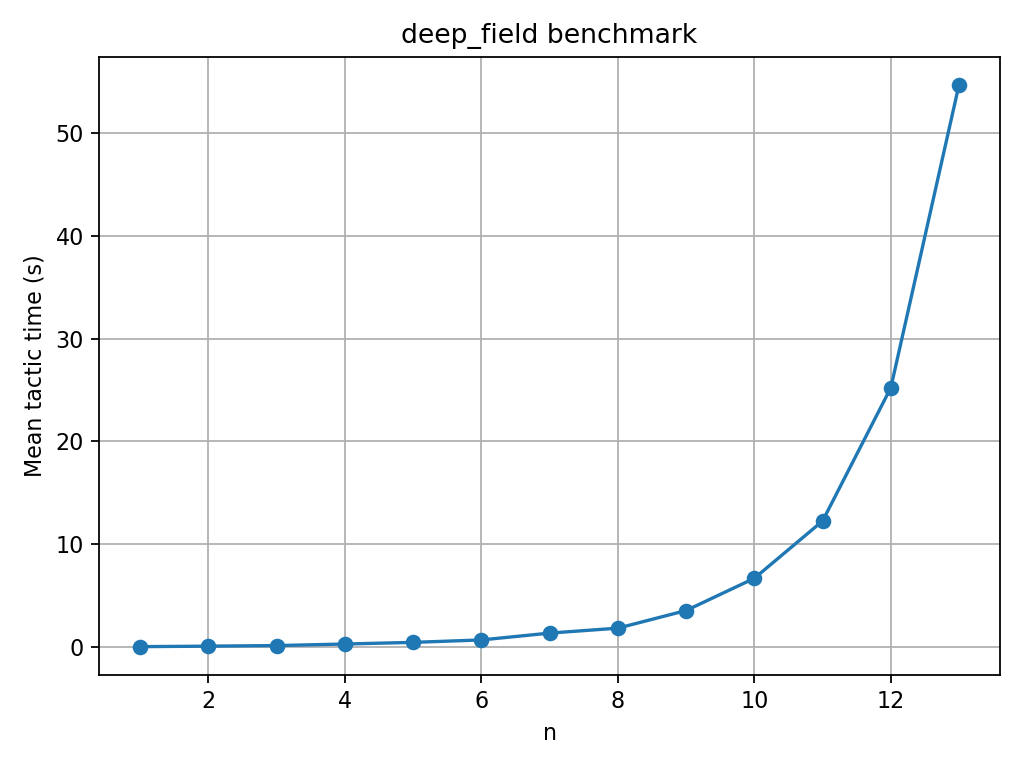
\includegraphics[width=0.8\textwidth]{images/benchmark.png}
  \caption{Measured execution times as a function of nesting depth $n$.}
  \label{fig:quadratic-fit}
\end{figure}
We evaluated 13 instances, for $(1 \leq n \leq 13)$, running each instance 10 times and reporting the mean execution time. The mean tactic execution time increased from (0.038) seconds at (n=1) to (54.715) seconds at (n=13), while the mean wall-clock time increased from (0.499) seconds to (74.090) seconds.

The execution time increases rapidly with the nesting depth. However, the practical relevance of this growth depends on the depths encountered in actual proofs. For undergraduate mathematical students it is unlikely to encounter more than say depth 5 formula, so the cost is acceptable.


\section{Lessons learned}
The implementation separates polynomial computation from proof construction. The OCaml oracle proposes polynomial factors, while Rocq verifies the algebraic identities needed to justify their use. This separation allows the extension to benefit from external computation without trusting the OCaml implementation for correctness.

The experiment also highlights an important difference between deep ring and
deep field simplification. For ring expressions, normalization naturally
provides a canonical polynomial representation, so recursively simplifying
function arguments is sufficient to make equivalent terms syntactically
equal. For field expressions, equality can instead be established by cross
multiplication without producing such a common representation. The gcd
computation addresses this additional representation problem by making it possible to reduce the fraction.

The current extension nevertheless operates at a limited point in the field
simplification process. It handles the field expression selected by the
existing field-simplification infrastructure, but it does not yet recursively
traverse arbitrary nested field expressions in the same way as the deep ring
procedure. A fully general deep field simplification procedure would therefore
require extending the recursive traversal.

% \section{Future work}

% Several extensions remain possible:

% \begin{itemize}
% \item extending the gcd-based reduction to a general deep field
% simplification procedure;
% \item improving the staging of normalization and rewriting to avoid
% unnecessary computation;
% \item reducing the number of generated proof obligations;
% \item extending deep ring and field reasoning to expressions involving
% exponents;
% \item exploring similar techniques for commutative-group isomorphisms;
% \item strengthening the polynomial gcd computation to support a broader
% range of integer representations.
% \end{itemize}


\section{Conclusion}

Extending reflexive algebraic tactics to expressions occurring inside
unrecognized function applications requires more than recursively invoking
the existing normalization procedures. For ring expressions, polynomial
normalization already provides a canonical representation that can be
propagated through the surrounding function application. For field
expressions, cross multiplication can prove equality without producing such a
representation, so an additional reduction step is required.

This work uses a polynomial gcd computation to provide that reduction. An
OCaml oracle computes the common factor and the corresponding numerator and
denominator quotients, while Rocq verifies the resulting factorization
identities and side conditions. ELPI provides the interface between the
external computation and the existing Ltac and field-simplification
infrastructure.

A natural next step is to extend the approach to a general deep field-simplification procedure that processes nested expressions from the inside out. This could also reduce unnecessary computation and the number of generated side conditions, but its effectiveness must be evaluated experimentally. Measurements of proof success, execution time, and generated side conditions would help assess the practical benefits of the approach.

The broader objective is to make algebraic automation behave more
naturally on mathematical expressions, while preserving the
proof guarantees of Rocq. The combination of recursive
simplification, polynomial factorization, and proof-producing
normalization provides a foundation for pursuing this objective
beyond the ring and field fragments.

\bibliographystyle{plain}
\bibliography{references}
\end{document}
